\section{An\'alisis de resultados}

\subsection{High-pass}

Se muestra la respuesta calculada, simulada y medida en la figura \ref{fig:ej2_HP_bode}. La respuesta calculada se separa de la simulada y la medida en los mismos rangos en que la imepdancia de entrada del gyrator calculada se separa de la simulada.

\begin{figure*}
	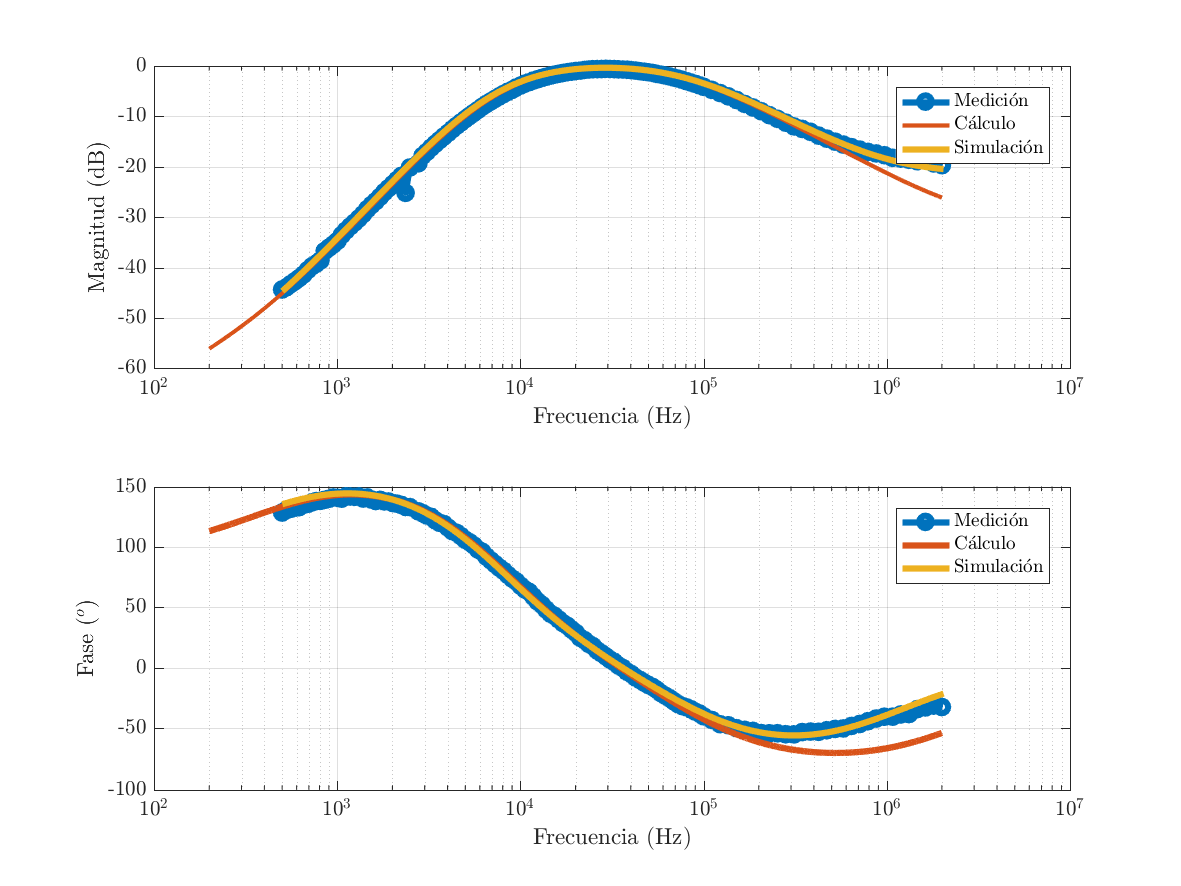
\includegraphics[width=0.7\textwidth]{imagenes/HP_bode}
	\caption{Respuesta en frecuencia del filtro high-pass calculada, simulada, y medida}
		\label{fig:ej2_HP_bode}
\end{figure*}

%\subsection{Low-pass}
%\ref{fig:ej2_LP_bode}
%\begin{figure*}
%	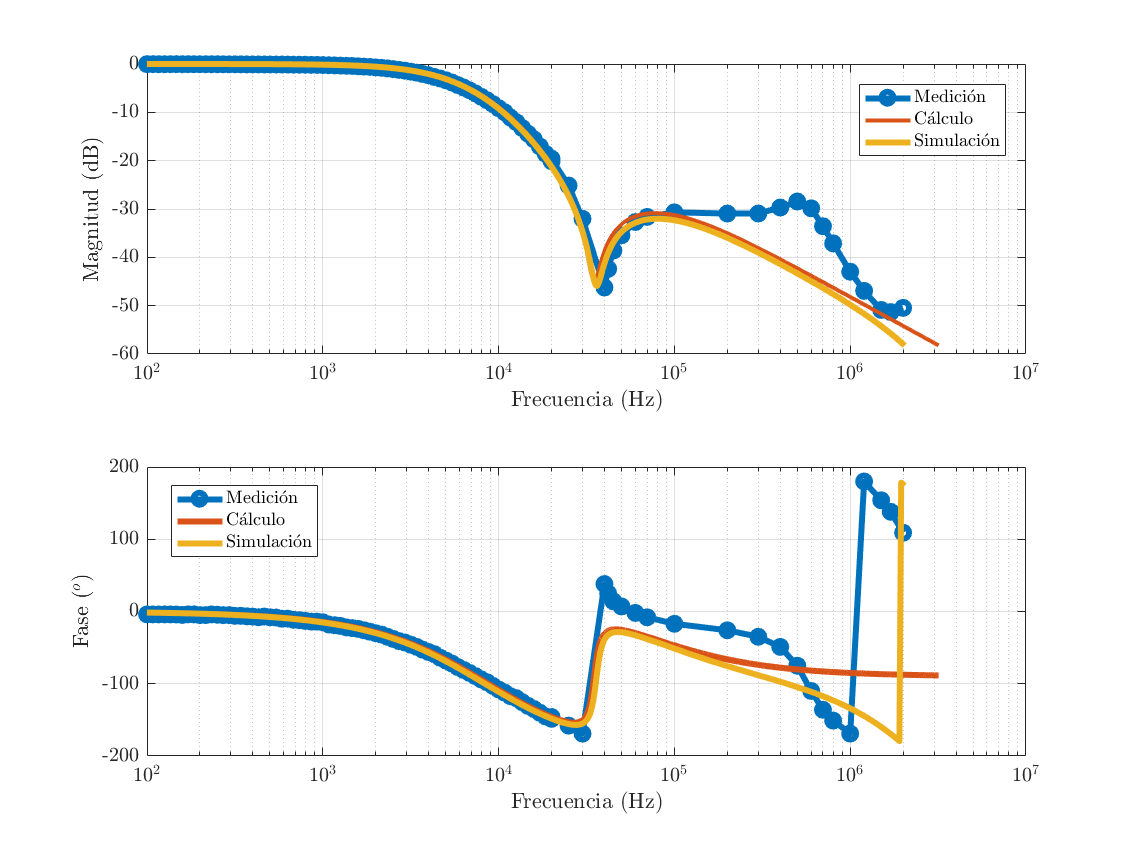
\includegraphics[width=\textwidth]{imagenes/LP_bode}
%	\caption{Respuesta en frecuencia del filtro low-pass calculada, simulada, y medida. El caculo fue hecho para salida diferencial, y la simulacion y la medicion para la salida del restador}
%		\label{fig:ej2_LP_bode}
%\end{figure*}


\subsection{Band-pass}

Se muestra la respuesta calculada, simulada y medida en la figura \ref{fig:ej2_BP_bode}. La respuesta calculada no se separa de la simulaci\'on como si lo hacia la del high-pass, ya que en ese rango de frecuencias el valor del paralelo de capacitor y el inductor esta dominado por el capacitor.

\ref{fig:ej2_BP_bode}
\begin{figure*}
	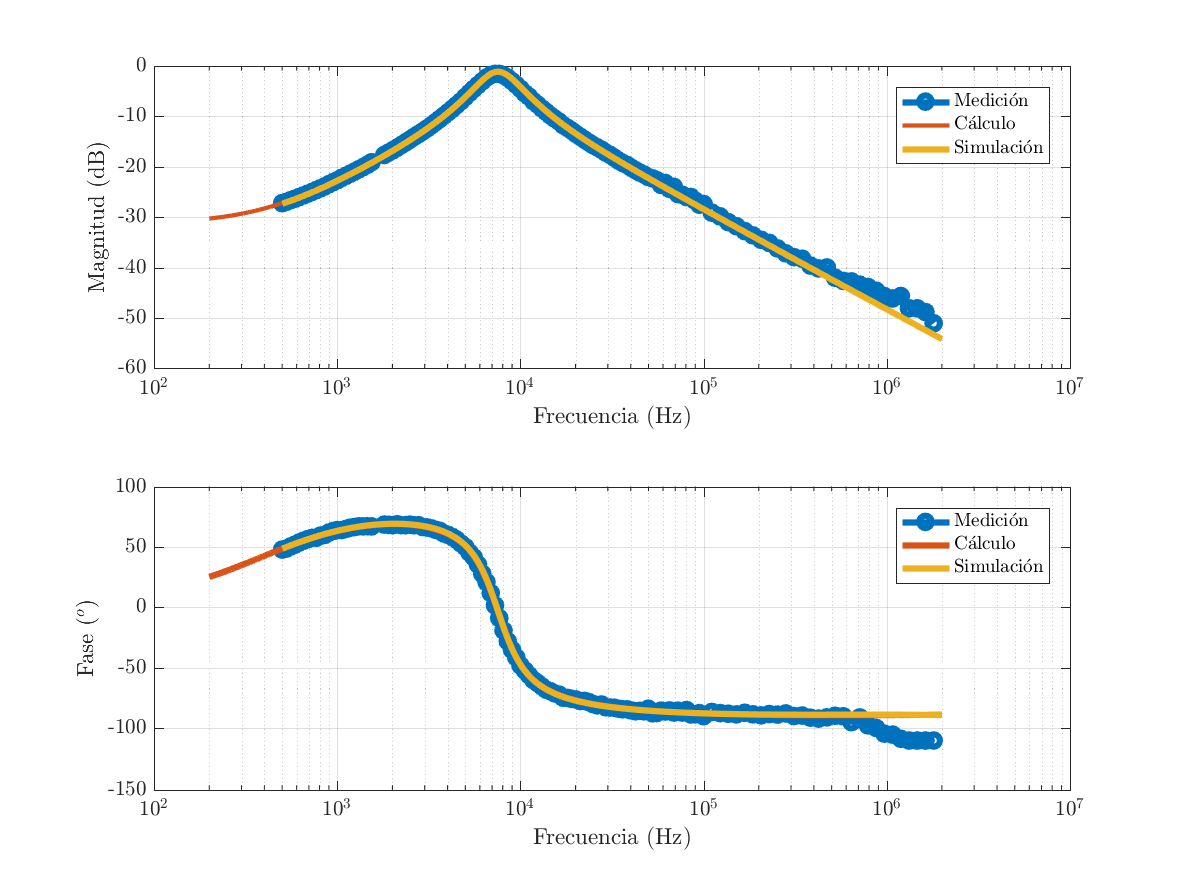
\includegraphics[width=0.7\textwidth]{imagenes/BP_bode}
	\caption{Respuesta en frecuencia del filtro band-pass calculada, simulada, y medida}
		\label{fig:ej2_BP_bode}

\end{figure*}


\subsection{Band-reject}

Se muestra la respuesta calculada, simulada y medida en la figura\ref{fig:ej2_BR_bode}. Se repite la diferencia de comportamiento entre la respuesta calculada, y la simulada y medida del filtro high-pass. 
\begin{figure*}
	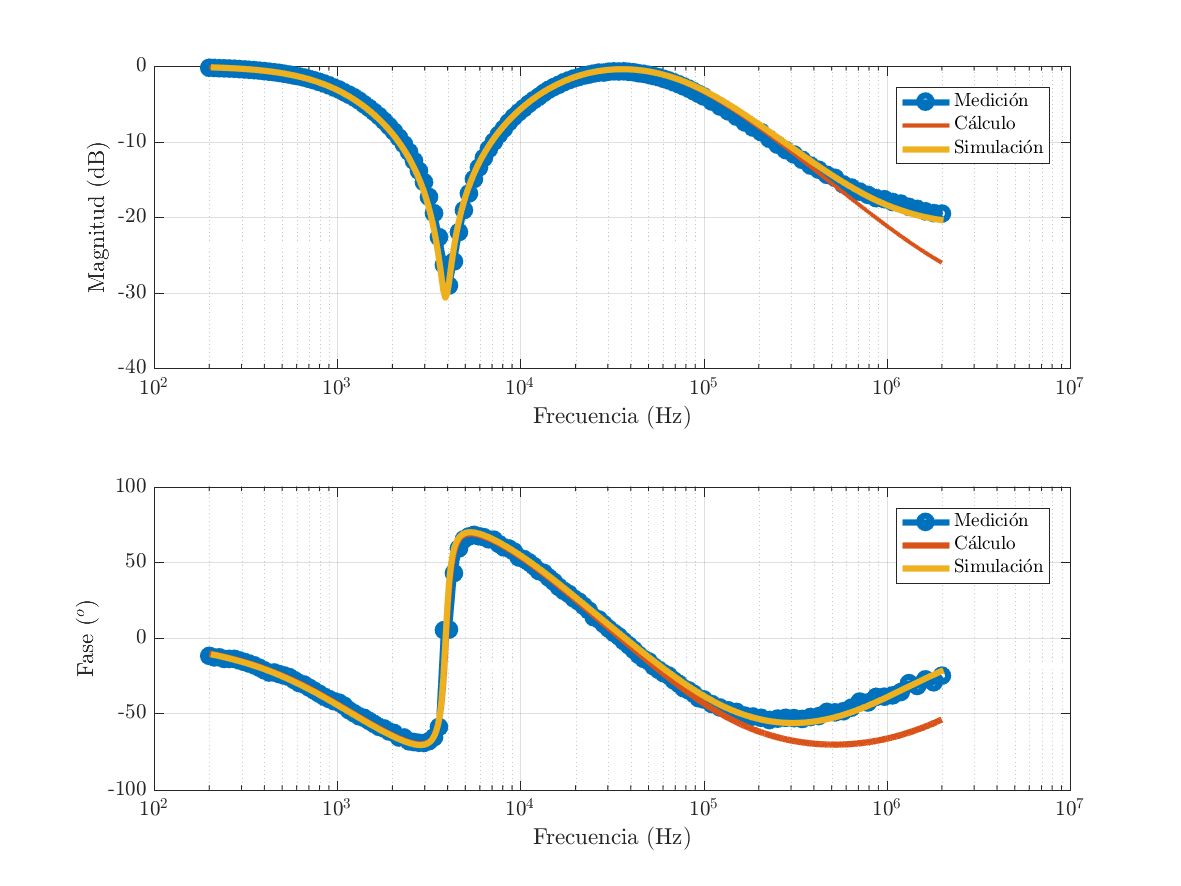
\includegraphics[width=0.7\textwidth]{imagenes/BR_bode}
	\caption{Respuesta en frecuencia del filtro band-reject calculada, simulada, y medida}
		\label{fig:ej2_BR_bode}

\end{figure*}

